\begin{ledgroupsized}[r]{120mm}
\footnotesize
\pstart
\noindent\textbf{\"{U}berlieferung:}
\pend
\end{ledgroupsized}
\begin{ledgroupsized}[r]{114mm}
\footnotesize
\pstart
\parindent -6mm
\makebox[6mm][l]{\textit{L}}Konzept: LH XXXV 9, 11 Bl. 5-8. 2 Bog. 2\textsuperscript{o}. 7 \nicefrac{1}{2} S. Die untere H\"{a}lfte von Bl. 8~v\textsuperscript{o} überliefert N.~34\textsubscript{2}.
Im oberen Drittel von Bl.~7~r\textsuperscript{o} finden sich gestrichene Rechnungen,
die mit dem sonst fortlaufenden Text nicht zusammenh\"{a}ngen (sie werden in \textit{LSB} VII ediert).
Auf Bl. 5~r\textsuperscript{o} und Bl.~8~r\textsuperscript{o} ist jeweils eine gestrichene Zeichnung anzutreffen;
beide werden im Folgenden nicht ber\"{u}cksichtigt, weil sie lediglich erste Versuche zu [\textit{Fig. 2}] bzw. [\textit{Fig. 6}] darstellen.
Leibniz' eigenh\"{a}ndige Datierung und Nummerierung der Bogen:
\textit{May 1675. Frottement. Part. (1)} am oberen Rand von Bl. 5~r\textsuperscript{o};
\textit{May 1675. Frottement part. (2)} am oberen Rand von Bl. 7~r\textsuperscript{o}.
Gleicher Wasserzeichentypus auf Bl.~6 und Bl.~8.
Der Text wird editorisch in drei Teile unterteilt, die auf verschiedene Redaktionsstufen zur\"{u}ckgehen k\"{o}nnten.%
\\Cc 2, Nr. 965 A, H, B, G, C
\pend
\end{ledgroupsized}
\newpage
\pstart
\noindent
[5~r\textsuperscript{o}] May 1675.
\pend
\pstart
\begin{center}
%\vspace*{0,5em} 
De la retardation du mouuement par le frottement
\end{center}
\pend
%\vspace*{-4mm}
\pstart
\begin{center} [\textit{Teil 1}]
\end{center}
\pend
\count\Afootins=1200
\count\Bfootins=1200
\count\Cfootins=1200
\pstart
\textso{Definition}
\pend
\begin{Geometrico}
\textso{Frottement }est un attouchement continuel, d'un corps qui est en mouuement, \`{a} un autre qui ne l'est pas, ou qui l'est autrement.
\end{Geometrico}
\begin{Geometrico}
\textso{Observation:} tout
\edtext{frottement des corps sensibles retarde leur mouuement}{\lemma{frottement}\Bfootnote{\textit{(1)}\ retarde le mouuement \textit{(2)}\ des corps [...] mouuement \textit{L}}}.
\end{Geometrico}
\pstart
Car nous voyons par
\edtext{experience, qu'un corps qui glisse ou qui roule sur un autre[,] [quelques polis]\edtext{}{\Bfootnote{quelque poli\textit{\ L \"{a}ndert Hrsg.}}} qu'ils puissent estre[,] va bien moins viste, que s'il estoit m\^{u} \`{a} travers de l'air,}
{\lemma{experience}\Bfootnote{\textit{(1)}\ qu'un corps \textit{(a)}\ quoyque \textit{(b)}\ uni \textit{(c)}\ bien poli,  \textit{(aa)}\ ne laisse pas de perdre une  \textit{(aaa)}\ vites \textit{(bbb)}\ partie \textit{(bb)}\ perd sa vitesse\protect\index{Sachverzeichnis}{vitesse} plus tost sur un plan quelque  \textit{(aaa)}\ poli \textit{(bbb)}\ uni qu'il puisse estre, que dans l'air. \textit{(2)}\ que les corps qui \textit{(3)}\ qu'un [...] autre[,]  \textit{(a)}\ quelque  \textit{(aa)}\ poli \textit{(bb)}\ uni qu'il puisse estre \textit{(b)}\ [quelques polis] [...] estre[,]  \textit{(aa)}\ laisse bien plus tost \textit{(bb)}\ va bien [...] estoit m\^{u}  \textit{(aaa)}\ sans aucun support, \textit{(bbb)}\ \`{a} travers de l'air, \textit{L}}}
suspendu d'un fil. Et nous reconnoissons que les liqueurs retardent beaucoup le mouuement des corps; et qu'une plume tombe
\edtext{bien moins}{\lemma{bien}\Bfootnote{\textit{(1)}\ plus \textit{(2)}\ moins \textit{L}}}
viste dans l'air que dans le vuide\protect\index{Sachverzeichnis}{vide}. Il ne s'agit pas \`{a} present d'en chercher la cause en supposant que les  \edtext{corps font des enfonceures}{\lemma{corps}\Bfootnote{\textit{(1)}\ enfoncent \textit{(2)}\ font des enfonceures \textit{L}}}
dans\hfill  les\hfill  plans\hfill  sur\hfill  lesquels\hfill  ils\hfill  marchent,\hfill  ou\hfill  que\hfill  les\hfill  plans\hfill  sont\hfill  \^{a}pres\hfill  et
\pend
\vspace{2.5em} 
\pstart
%\vspace{1em} 
\noindent
\begin{minipage}[c]{0.5\textwidth}
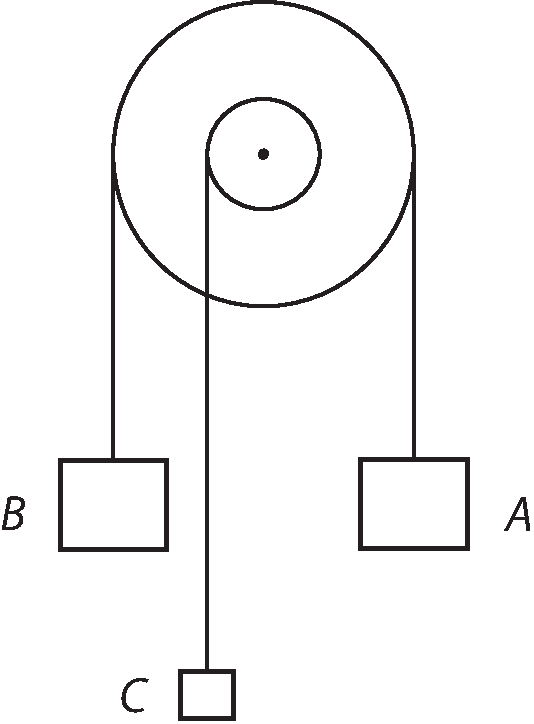
\includegraphics[trim = -30mm -8mm -5mm 0mm, clip, width=0.8\textwidth]{images/lh0350911_005r-d1.pdf}
\end{minipage}
\hspace*{13,3mm}
\begin{minipage}[c]{0.5\textwidth}
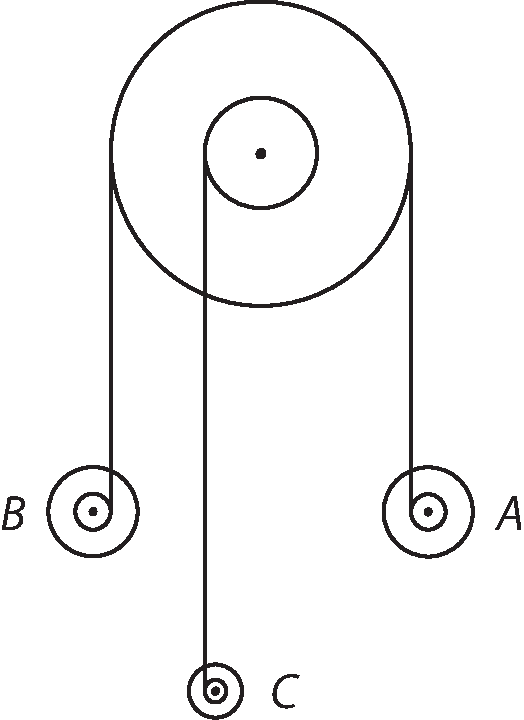
\includegraphics[trim = 0mm -8mm -5mm 0mm, clip, width=0.61\textwidth]{images/lh0350911_005r-d2.pdf}
\end{minipage}
%\vspace*{1mm}
\hspace*{25mm} [\textit{Fig. 1}]\hspace*{57mm} [\textit{Fig. 2}]
%\vspace*{1em}
\pend
%\newpage
\pstart \noindent raboteux, et pleins d'une infinit\'{e} de pointes pliables \edtext{et \`{a} ressort,}{\lemma{et \`{a} ressort}\Bfootnote{\textit{erg. L}}}
\edtext{dont la pluspart}{\lemma{dont}\Bfootnote{\textit{(1)}\ une partie \textit{(2)}\ la pluspart \textit{L}}}
cede et se remet et quelques unes se cassent.
Car il suffit icy d'estre asseur\'{e} du fait, et d'en tirer des consequences incontestables.
\pend
\count\Bfootins=1000
\count\Afootins=1000
\begin{Geometrico}
\textso{Axiome de Mechanique:}\edtext{ Differentes}{\lemma{\textso{Mechanique:}}\Bfootnote{\textit{(1)}\ Les \textit{(2)}\ Differentes \textit{L}}}
\edtext{resistences\protect\index{Sachverzeichnis}{r\'{e}sistance} d'une certaine force \`{a} quelque changement
sont entre elles comme les vitesses des changemens qui arriveroient sans la resistence: par exemple}%
{\lemma{resistences}\Bfootnote{%
\textit{(1)}\ d'une m\^{e}me force \`{a} une m\^{e}me force sont entre elles comme les vistesses des %
\textbar\ m\^{e}mes \textit{erg} \textbar\ effects %
\textit{(a)}\ qui s'ensuivroient, si celle qui resiste %
\textit{(b)}\ opposez \`{a} celle qui resiste qui s'ensuivroient, si elle estoit surmont\'{e}e %
\textit{(2)}\ d'une \textit{(a)}\ m\^{e}me \textit{(b)}\ certaine [...] sont %
\textbar\ entre elles \textit{erg.} \textbar\ comme les vitesses %
\textit{(aa)}\ par exemple: %
\textit{(bb)}\ des changemens  %
\textit{(aaa)}\ qui devroient %
\textit{(aaaa)}\ suivre \textit{(bbbb)}\ arriver sans la %
\textit{(bbb)}\ qui [...] resistence %
\textit{(aaaaa)}\ caeteris paribus. %
\textit{(bbbbb)}\ : par exemple \textit{L}}}
\edtext{soit consider\'{e}e}{\lemma{soit}\Bfootnote{\textit{(1)}\ un poids \textit{(2)}\ consider\'{e}e \textit{L}}}
\edtext{une force comme celle}{\lemma{force}\Bfootnote{\textit{(1)}\ qui resiste \textit{(2)}\ comme celle \textit{L}}}
du poids\protect\index{Sachverzeichnis}{poids} $\displaystyle A$ qui resiste \`{a} estre lev\'{e} en haut;
soit une autre force, comme celle \edtext{du poids}{\lemma{du}\Bfootnote{\textit{(1)}\ corps \textit{(2)}\ poids \textit{L}}}
$\displaystyle B$
\edtext{ou $\displaystyle C$}{\lemma{ou $\displaystyle C$}\Bfootnote{\textit{erg. L}}}
appliqu\'{e}e \`{a} la premiere, en sorte, qu'elle luy devienne oppos\'{e}e, et qu'elle s'efforce
\edtext{de lever le poids $\displaystyle A$, et de vaincre}{\lemma{de}\Bfootnote{\textit{(1)}\ vaincre \textit{(2)}\ lever [...] vaincre \textit{L}}}
sa resistence. Je dis que \edtext{la resistence du  poids}{\lemma{la}\Bfootnote{ \textit{(1)}\ m\^{e}me force \textit{(2)}\ resistence  \textit{(a)}\ de la m\^{e}me force  \textit{(b)}\ du  \textbar\ m\^{e}me \textit{ gestr.}\ \textbar\  poids \textit{L}}}
$\displaystyle A$, quand il doit estre lev\'{e} subitement est \`{a} la resistence du \edtext{m\^{e}me poids}{\lemma{m\^{e}me}\Bfootnote{\textit{(1)}\ corps \textit{(2)}\ poids \textit{L}}}
quand il doit estre lev\'{e} doucement, en raison des vitesses
\edtext{dont il doit estre lev\'{e} \`{a} une m\^{e}me hauteur.}{\lemma{dont il}\Bfootnote{%
\textit{(1)}\ seroit lev\'{e}, et il %
\textit{(2)}\ doit estre lev\'{e} %
\textit{(a)}\ . Le m\^{e}me est vra %
\textit{(b)}\  \`{a} une m\^{e}me hauteur. \textit{L}}}%
\edtext{}{\lemma{}\Afootnote{\textit{Zwischen den Zeilen, gestrichen und abbrechend:} Chose dont tous ceux qui ont pens\'{e} sur la statique\vspace{0mm}}}
Et cela se trouue veritable aussi en substituant des ressorts
\edtext{\`{a} bander}{\lemma{\`{a} bander}\Bfootnote{\textit{erg. L}}}
\`{a} la place des poids \`{a} lever.
Je tiens cet axiome demontrable: mais il suffit de s'en servir \`{a} present comme d'un proposition avou\'{e}e de tous les s\c{c}avans, et reconnue par tous les
ouuriers.\edlabel{35.09.11_005r_01}%
\edtext{}{{\xxref{35.09.11_005r_01}{35.09.11_005r_02}}\lemma{ouuriers.}\Bfootnote{%
\textit{(1)}\ \textso{Consequence} de cet axiome %
\textit{(2)}\ \textso{Autre Axiome.} %
\textit{(a)}\ Toute la resistence surmont\'{e}e deminue le mouuement de la force qui l'a surmont\'{e}e %
\textit{(b)}\ Si un corps \textit{L}}}
\end{Geometrico}
\begin{Geometrico}
\textso{Autre Axiome.} Si un corps\edlabel{35.09.11_005r_02}
l'emporte \edtext{sur}{\lemma{sur}\Bfootnote{\textit{erg. L}}}
un \edtext{autre malgr\'{e} sa resistence, mais avec diminution de son propre mouuement}{\lemma{autre}\Bfootnote{\textit{(1)}\ mais avec diminution de son propre mo \textit{(2)}\ malgr\'{e} [...] mouuement \textit{L}}},
les diminutions seront en raison des vistesses\edtext{.}{\lemma{}\Afootnote{\textit{Zwischen den Zeilen:} Error\vspace{-4mm}}}
\end{Geometrico}
\pstart
\noindent
C'est \`{a} \edtext{dire si le m\^{e}me corps ou un pareil l'emporte}{\lemma{dire}\Bfootnote{%
\textit{(1)}\ si un autre corps %
\textit{(2)}\ si le m\^{e}me corps %
\textbar\ ou un pareil \textit{erg.} \textbar\ l'emporte \textit{L}}} encor une fois sur une m\^{e}me \edtext{ou \'{e}gale}{\lemma{}\Bfootnote{ou \'{e}gale \textit{erg.} \textit{L}}}
resistence, mais avec une autre vistesse; la premiere diminution de vitesse sera \`{a} la seconde, comme la premiere vitesse est \`{a} la seconde vitesse.
[5~v\textsuperscript{o}]
\pend
\count\Bfootins=1500
\count\Afootins=1500